\begin{mainquestion}{battery}{Battery Characteristics}

\questionpoints A typical CR2032 3V coin-style battery has an internal source resistance $R_s$ of about \SI{17}{\ohm} at room temperature. (While this value typically increases as the battery is depleted, we will consider it constant for this problem.)

\begin{center}
    \begin{circuitikz}[scale=1, american]
        % Added 'invert' to flip polarity
        \draw (0,0) to[V, l=$V_{batt}$, invert] (0,3) to[R, l=$R_s$] (3,3) to[short, -o] (4,3);
        \draw (0,0) to[short, -o] (4,0);
        \draw (4,3) to[R, l=$R_L$, i=$I_L$] (4,0);
    \end{circuitikz}
\end{center}

% =========================================================
\begin{partquestion}{peakcurrent}
{Using this battery, what is the peak current that could be driven through an external load $R_L$? What is $R_L$ in this scenario?}

\begin{answer}[1.5in]
        The current is $I_L = \frac{V_{batt}}{R_s + R_L}$.
        To make this as large as possible, we make the denominator as small as possible. With $R_s$ fixed, we make $R_L = \SI{0}{\ohm}$.
        So, 
        \[ I_L = \frac{V_{batt}}{R_s} = \frac{\SI{3}{\volt}}{\SI{17}{\ohm}} = \SI{176}{\milli\ampere}. \]
\end{answer}

\end{partquestion}

% =========================================================
\begin{partquestion}{peakpower}
{Using this battery, what is the peak power that could be delivered through an external load $R_L$? What is $R_L$ in this scenario?}

\begin{answer}[1.5in]
        Maximum power transfer occurs when $R_L = R_s = \SI{17}{\ohm}$ and the value of the power is:
        \[ P_L = \frac{V_L^2}{R_L} = \frac{(V_{batt}\frac{R_L}{R_L+R_s})^2}{R_L} = \frac{V_{batt}^2 R_L}{(R_L+R_s)^2} = \frac{V_{batt}^2}{4R_s} \]
        \[ = \frac{3^2}{4(17)} = \SI{132}{\milli\watt}. \]
\end{answer}

\end{partquestion}

% =========================================================
\begin{partquestion}{plotpower}
{Plot the power delivered to $R_L$ as a function of $R_L$, from 0 to \SI{500}{\ohm}.}

\begin{answer}[1.5in]
        In the previous part, we derived the formula for the power dissipated in the load as:
        \[ P_L = \frac{V_L^2}{R_L} = \frac{V_{batt}^2 R_L}{(R_L+R_s)^2} = \frac{9R_L}{(R_L+17)^2} \]
        This can be plotted using MATLAB or some equivalent graphing program.

        \begin{center}
            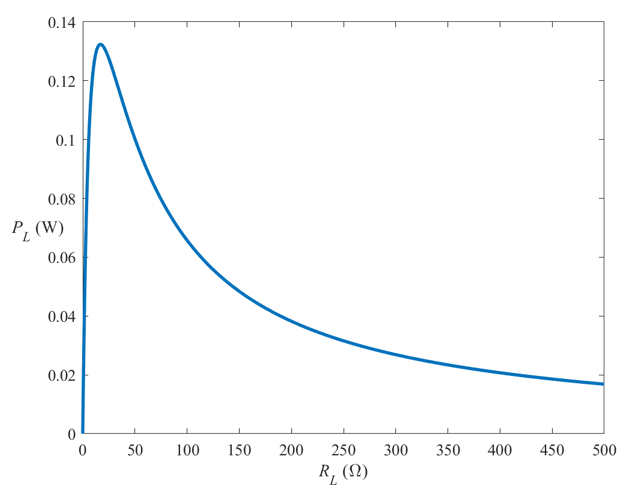
\includegraphics[width=0.7\textwidth]{battery_characteristics_graph.png}
        \end{center}
        
\end{answer}

\end{partquestion}

\end{mainquestion}
